\section{时序RDF图存储结构和查询引擎}
时序RDF图的存储主要是基于\S\ref{chap:kvstore}中介绍的分布式键值存储实现的,在此基础上,它还使用分布式排序数组结构加速时间条件查询。时序RDF图查询引擎使用存储层提供的接口、按照用户指定的查询计划执行SPARQL-T查询语句中GP的各模式。本节将详细介绍时序RDF图的存储结构和查询引擎。
\subsection{存储结构}
\label{sec:rdfstore}
如\S\ref{sec:arch}所述,\sys 并不直接存储时序RDF图数据集中的字符串,而是将其转化成整型ID进行存储,并使用字符串服务器管理字符串和整型ID之间的对应关系。时序RDF图数据集中的字符串分为两类:
\begin{enumerate}
\item 时序三元组中表示谓词的字符串及表示类型名的字符串,例如时序三元组\texttt{Eric memberOf X-Lab [1,2)}中的\texttt{memberOf}和时序三元组\texttt{Eric rdf:type Student [0,+$\infty$)}中的\texttt{rdf:type}、\texttt{Student}。
这类字符串对应的ID范围为$[1,2^{17})$,特别地,\texttt{rdf:type}对应的ID为1。
本文将表示谓词的字符串对应的ID称为\texttt{pid},将表示类型名的字符串对应的ID称为\texttt{tid}。
\item 时序三元组中表示主语和宾语的字符串(表示类型名的字符串除外),例如时序三元组\texttt{Eric memberOf X-Lab [1,2)}中的\texttt{Eric}和\texttt{X-Lab}。这类字符串对应的ID范围为$[2^{17},2^{46})$。本文将这类字符串对应的ID称为\texttt{vid}。
\end{enumerate}

系统默认使用32位UINT表示各种ID,对于规模比较庞大的数据集,可以在系统编译时指定使用64位UINT。

时序RDF图存储内存布局如图\ref{trdfstore},分为键值存储区和时序三元组存储区两部分。
时序三元组存储区本质上是内存数组,它分为两部分,在“时序三元组存储1”中,时序三元组按照有效时间区间的开始时间升序排布;在“时序三元组存储2”中,时序三元组按照有效时间区间的截止时间升序排布。
键值存储区中的键值对分为直接索引和间接索引两类,在直接索引中,值是实际数据;在间接索引中,值由指向“时序三元组存储1”中时序三元组的指针组成。

\begin{figure}[!htb]
\center{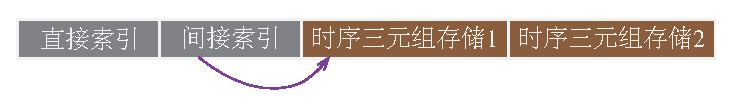
\includegraphics[width=0.6\textwidth]  {figures/trdfstore.eps}}
\bicaption{时序RDF图存储内存布局}{Temporal RDF graph storage memory layout}
\label{trdfstore}
\end{figure}

在键值存储区中,各种键值对及其类型如表\ref{tab:trdf}所示。键的数据类型是64位UINT,由三部分组成,第一部分使用其高46位,第二部分使用其中间17位,第三部分使用其最低位。第三部分只能是OUT(1,表示出方向)和IN(0,表示入方向)其中之一。值的基本数据类型与ID的数据类型相同,可以是32或64位UINT,这取决于系统编译时的配置。
\begin{table}[!hpt]
  \bicaption{时序RDF图存储使用的键值对}{Key-value pairs used in temporal RDF graph storage}
  \label{tab:trdf}
  \centering
  \begin{tabular}{p{1cm}p{3cm}p{8cm}p{2cm}} \toprule
    序号 & 键 & 值 & 类型 \\ \midrule
    1\centering & \texttt{[0|0|OUT]} & 所有\texttt{pid} & \multirow{8}{*}{直接索引} \\
    2\centering & \texttt{[0|1|OUT]} & 所有\texttt{tid} & \\
    3\centering & \texttt{[0|1|IN]} & 所有\texttt{vid} & \\
    4\centering & \texttt{[0|tid|IN]} & 所有类型为\texttt{tid}的\texttt{vid} & \\
    5\centering & \texttt{[0|pid|OUT]} & 谓词为\texttt{pid}的所有时序三元组中所有表示宾语的\texttt{vid} & \\
    6\centering & \texttt{[0|pid|IN]} & 谓词为\texttt{pid}的所有时序三元组中所有表示主语的\texttt{vid} & \\
    7\centering & \texttt{[vid|0|OUT]} & 主语为\texttt{vid}的所有时序三元组中的所有\texttt{pid} & \\
    8\centering & \texttt{[vid|0|IN]} & 宾语为\texttt{vid}的所有时序三元组中的所有\texttt{pid} & \\ 
    \hline
    9\centering & \texttt{[vid|1|OUT]} & 描述\texttt{vid}类型的时序三元组 & \multirow{3}{*}{间接索引} \\ 
    10\centering & \texttt{[vid|pid|OUT]} & 主语为\texttt{vid}、谓词为\texttt{pid}的所有时序三元组 & \\ 
    11\centering & \texttt{[vid|pid|IN]} & 宾语为\texttt{vid}、谓词为\texttt{pid}的所有时序三元组 & \\ 
    \bottomrule
  \end{tabular}
\end{table}

图\ref{trsdemo}给出了系统会为图\ref{trdf}中的数据集生成的一部分键值对。为了便于理解,图中使用字符串表示主语、谓词和宾语,系统实际使用的是这些字符串对应的ID。
在间接索引中,值是一个由时序三元组在“时序三元组存储1”中的偏移量组成的列表,例如,时序三元组\texttt{Kurt memberOf X-Lab [1,4)}在“时序三元组存储1”中的偏移量为5,那么间接索引就使用5来表示该时序三元组。

\begin{figure}[!htb]
\center{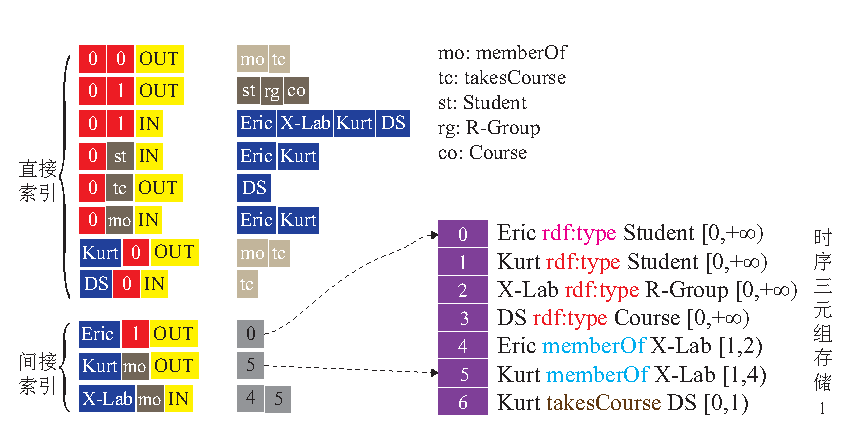
\includegraphics[width=0.75\textwidth]  {figures/trsdemo.eps}}
\bicaption{时序RDF图存储使用的键值对示例}{Example of key-value pairs used in temporal RDF graph storage}
\label{trsdemo}
\end{figure}

为了实现RDF数据集的分布式可扩展存储,系统使用如下规则将键值对和时序三元组划分到各查询节点中存储:
\begin{enumerate}
    \item 每个查询节点负责一部分\texttt{vid}的管理,\texttt{vid}会被分配到的查询节点(查询节点从0开始编号)为:
    \begin{equation}
        \mathtt{vid \ \% \ num\_qnodes}
    \end{equation}
    其中\texttt{num\_qnodes}是查询节点数。
    \item 对于键值对1-6,将值按照1中的规则划分到各查询节点存储,同一键会出现在每个查询节点的键值存储中;对于键值对7-11,将键依据其第一部分按照1中的规则划分到不同查询节点存储,每个键只会出现在一个查询节点的键值存储中。
    \item 将所有时序三元组分别按有效时间区间的开始时间和截止时间排序后,分别按块划分到各查询节点的“时序三元组存储1”和“时序三元组存储2”中存储,偏移量为\texttt{off}的时序三元组会被分配到的查询节点(从0开始编号)为:
    \begin{equation}
        \mathtt{off \ / \ \lceil num\_ttriples \ / \ num\_qnodes \rceil}
    \end{equation}
    其中\texttt{num\_ttriples}是时序三元组总数。
\end{enumerate}

分布式键值存储结构可以实现高效的拓扑查询,两个“时序三元组存储”可以实现高效的时间条件查询。对于以时序三元组有效时间区间开始时间为条件的查询,可以在“时序三元组存储1”上通过二分法快速找到目标时序三元组,同理可以使用“时序三元组存储2”快速处理以时序三元组有效时间区间截止时间为条件的查询。直接索引和间接索引相结合的键值存储结构可以在实现高效的拓扑查询和时间条件查询的同时,减少时序数据存储占用的空间。

表\ref{tab:storeif}列出了存储层向上提供的接口,接口\ding{182}只涉及对本节点上键值存储结构的读,接口\ding{183}可能涉及对各节点的键值存储结构和“时序三元组存储1”的读,接口\ding{184}和\ding{185}可以分别筛选出本节点的“时序三元组存储1”和“时序三元组存储2”中符合时间条件的时序三元组。
\begin{table}[!hpt]
  \bicaption{时序RDF图存储提供的接口}{Interfaces provided by temporal RDF graph storage}
  \label{tab:storeif}
  \centering
  \begin{tabular}{p{1cm}p{8cm}p{5.5cm}} \toprule
    序号 & 接口 & 作用 \\ \midrule
    \ding{182}\centering & \texttt{list<value\_t> get\_values(key)} & 获取本节点上键\texttt{key}对应的值列表,适用于键值对1-6 \\
    \ding{183}\centering & \texttt{list<triple\_t> get\_ttriples(key)} & 获取键\texttt{key}对应的时序三元组列表,适用于键值对7-11 \\
    \hline
    \ding{184}\centering & \texttt{list<triple\_t> get\_ttriples\_ts(start, end)} & 从本节点的“时序三元组存储1”中获取所有有效时间区间开始时间范围为\texttt{[start,end]}的时序三元组 \\
    \ding{185}\centering & \texttt{list<triple\_t> get\_ttriples\_te(start, end)} & 从本节点的“时序三元组存储2”中获取所有有效时间区间截止时间范围为\texttt{[start,end]}的时序三元组 \\
    \bottomrule
  \end{tabular}
\end{table}

\subsection{查询引擎}
SPARQL-T查询引擎沿用了Wukong使用的图探索和全历史剪枝算法。
默认情况下,查询引擎会使用存储层提供的接口\ding{182}和\ding{183}通过键值存储查找所需的数据,但对于一些以时间点或时间范围为条件的查询,通过接口\ding{184}和\ding{185}直接从“时序三元组存储”中寻找符合条件的时序三元组可能更加高效。
例如图\ref{tsparql}中的查询语句想要找到满足如下条件的资源Y:Y的类型是课程且有加入X-Lab时间为1的X-Lab成员选修该课程。
在执行该语句时,可以先在“时序三元组存储1”中快速找到有效时间区间开始时间为1的时序三元组,然后再对这些时序三元组做进一步筛选。如果查询引擎不直接使用“时序三元组存储”,而是先使用键值存储做图探索,然后再筛选出变量\texttt{ts}的取值为1的查询结果,那么就会带来更大的数据访问开销。用户可以通过在GP中使用\textbf{时序三元组时间范围模式}显式地要求查询引擎使用“时序三元组存储”进行时间条件查询,语法为:
\begin{equation}
    \mathtt{interval \ s \ p \ o \ STRAT/END(const_1, const_2)}
\end{equation}
其中\texttt{s}、\texttt{p}和\texttt{o}分别表示时序三元组的主语、谓词和宾语,它们都可以是常量或变量;\texttt{interval}是可选的,它是一个由两个变量组成的区间,格式为\texttt{[?var$_1$,?var$_2$)},当它存在时,两个变量会分别取值为查询到的时序三元组的有效时间区间的开始时间和截止时间;\texttt{START}和\texttt{END}二选一,\texttt{START}指定依据有效时间区间开始时间进行查找,\texttt{END}指定依据有效时间区间截止时间进行查找;\texttt{const$_1$}和\texttt{const$_2$}是两个时间常量且\texttt{const$_1\leq$const$_2$},用于指定要查找的时间范围。
值得注意的是,用户需要自行估算使用时序三元组时间范围模式是否能够提高查询的执行效率,避免出现负优化。
图\ref{trp}中的查询语句与图\ref{tsparql}中的查询语句含义相同,但它显式地指定使用“时序三元组存储1”进行时间条件查询。

\begin{figure}[!htb]
\center{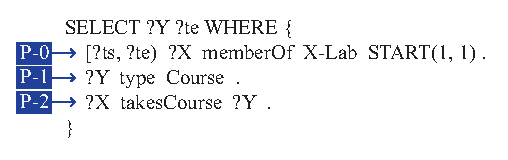
\includegraphics[width=0.55\textwidth]  {figures/trp.eps}}
\bicaption{显式指定使用“时序三元组存储”的查询语句示例}{Example of a query that explicitly specifies the use of "temporal triple storage"}
\label{trp}
\end{figure}

由于一条SPARQL-T查询语句可能包含多个五元模式或时序三元组时间范围模式,使用不同的顺序执行这些模式的效率可能不同,例如图\ref{trp}中的查询语句可以以以下两种不同的顺序执行:
\begin{itemize}
    \item 顺序一:
    \begin{itemize}
        \item 利用“时序三元组存储1”寻找变量\texttt{X}和\texttt{te}的所有可取值(P-0)
        \item 对于每行中间结果,从变量\texttt{X}的取值\texttt{val(X)}出发使用键\texttt{[val(X)| takesCourse|OUT]}找到变量\texttt{Y}的所有可取值(P-2)
        \item 对于每行中间结果,从变量\texttt{Y}的取值\texttt{val(Y)}出发使用键\texttt{[val(Y)| 1|OUT]}获取变量\texttt{Y}的类型,如果是\texttt{Course},则保留该行中间结果(P-1)
    \end{itemize}
    \item 顺序二:
    \begin{itemize}
        \item 利用“时序三元组存储1”寻找变量\texttt{X}和\texttt{te}的所有可取值(P-0)
        \item 使用键\texttt{[0|Course|IN]}找到变量\texttt{Y}的所有可取值(P-1)
        \item 对于每行中间结果,从变量\texttt{X}的取值\texttt{val(X)}出发使用键\texttt{[val(X)| takesCourse|OUT]}找到变量\texttt{Y}的可取值,如果其中包含变量\texttt{Y}的取值,则保留该行中间结果(P-2)
    \end{itemize}
\end{itemize}

由于系统并未实现SPARQL-T的执行优化器,无法自动确定最优的执行方案,所以需要用户在发起查询请求时通过自定义的查询计划指定查询引擎执行各模式的顺序。
另外,如果查询语句中包含时序三元组时间范围模式,查询引擎会先执行时序三元组时间范围模式,再执行五元模式。

SPARQL-T查询语句可分为大查询和小查询两类,大查询通常从大量顶点出发,探索庞大数量的路径,这一过程往往会访问时序RDF图中的很大一部分数据;小查询通常从一个固定的顶点开始,访问少量的路径和顶点。具体来说,大查询包含以下两类:
\begin{enumerate}
    \item 第一个查询模式需要用到键值对1-6的查询语句
    \item 包含时序三元组时间范围模式的查询语句
\end{enumerate}
其他的查询语句都属于小查询。

查询引擎使用fork-join机制来处理大查询。
工作线程在收到代理线程发来的大查询时,会将其分成\texttt{num\_qnodes} $\times$ \texttt{parallel\_factor}个子查询,然后分别发送给各个查询节点的\texttt{parallel\_factor}个工作线程共同执行,最后原工作线程负责子查询结果的合并。\texttt{parallel\_factor}是并行因子,其值越大,查询执行的并发度越高。

图\ref{fork-join}展示了一个大查询的fork-join过程,该查询的第一个查询模式需要使用键值对6。由于键值对6的值会被划分到所有查询节点存储,所以不同查询节点上读取到的键\texttt{[0|memberOf|IN]}对应的值是无共享的。同一查询节点上的不同工作线程读取到的值是相同的,工作线程会根据其线程号使用值列表中的一部分元素。
\begin{figure}[!htb]
\center{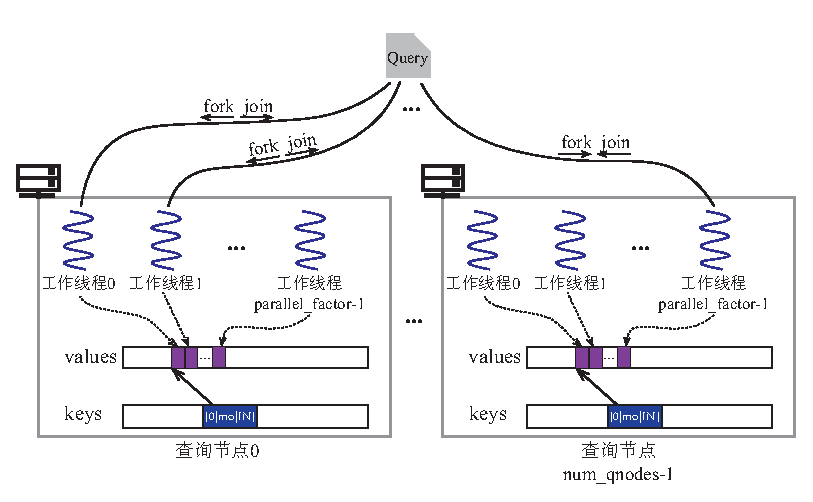
\includegraphics[width=0.75\textwidth]  {figures/fork-join.eps}}
\bicaption{大查询的fork-join过程}{Fork-join process of a heavy query}
\label{fork-join}
\end{figure}

查询引擎在处理小查询时也可能会使用fork-join机制:当工作线程在准备开始执行一个五元模式时,如果中间结果条目数达到系统预设的阈值(例如100),且工作线程需要通过较多跨节点的单边RDMA Read操作来执行该模式,那么工作线程会将其分成\texttt{num\_qnodes}个子查询,然后分别发送给各个查询节点的一个工作线程共同执行。查询的划分实质上是中间结果的划分,中间结果是依据执行该五元模式需要使用的变量的取值划分的,如果某行中间结果中该变量的取值为\texttt{val},那么该行中间结果会被划分到的子查询(从0开始编号)为:
\begin{equation}
    \mathtt{val \ \% \ num\_qnodes}
\end{equation}
查询划分完成后,子查询$i$会被发送到查询节点$i$执行。

只要遵守以上规则,子查询可以被进一步地划分,这样就可能形成一颗以代理线程发来的查询为根节点的查询树。

查询语句执行过程中,一个变量可能处于Unknown和Known两种状态,它们的含义分别为:
\begin{itemize}
    \item Unknown:该变量没有在之前的模式中出现过,当前中间结果表中没有该变量对应的列;
    \item Known:该变量已经在之前的模式中出现过,当前中间结果表中有该变量对应的列。
\end{itemize}

查询引擎在执行时序三元组时间范围模式时,会先从“时序超边存储”中查找所有符合模式指定的时间范围的时序三元组,然后逐一判断每个时序三元组是否与模式的前半部分(即\texttt{interval s p o})匹配。匹配一个时序三元组的方法为:先从\texttt{s}开始,如果它是变量且状态是Unknown,那么该时序三元组的主语就是它的一个可取值;如果它是变量且状态是Known,那么就需要逐一验证中间结果表每一行中该变量对应的列是否与该时序三元组的主语相同,若是则保留该行,否则舍弃该行;如果它是常量,那么只有在该时序三元组的主语与之相同时才可继续匹配。接着以类似过程匹配\texttt{p}、\texttt{o}、\texttt{interval}的\texttt{?var$_1$}和\texttt{?var$_2$}。

查询引擎在执行五元模式时,通常会先从其中的常量开始,通过构造合适的键从分布式键值存储中为模式中的变量寻找可取值,从而将变量的状态从Unknown转移到Known。然后可能会使用中间结果表每一行中Known变量对应的列的值继续构造合适的键进行进一步的图探索,直到所有五元模式都执行完毕。
